\documentclass[final]{beamer}
  \mode<presentation>
  {\usetheme{GMU}}


% Files needed are:
%    beamerposter-exampleSMU.tex (this file)
%    beamerthemeGMU.sty
%    beamerposter.sty
%
% Personal information that is in the footer is declared in the style file (very bottom of beamerthemeGMU.sty).
%
% Dimensions are given in cm such that the default of 160x120 = 4x3
%
% Compile with
%    latex filename.tex
%    dvips filename.dvi -o
%    ps2pdf filename.ps


\usepackage{times}
\usepackage{amsmath,amssymb, graphicx, braille}
\usepackage[english]{babel}
\usepackage[latin1]{inputenc}
\usepackage[orientation=landscape,size=custom,width=127,height=76.2,scale=2,debug]{beamerposter}  
  \title[Fancy Posters]{Contextual Machine Learning Through the Analysis and Chunking of Partially Translated Grade 2 Braille}
  \author[author]{Catherine Ray}
  \institute[George Mason University]{Dr. Muffarah Jahangeer, Dr. Joseph Marr}
%  \date{Jul. 31th, 2007}
  
%%%%%%%%%%%%%%%%%%%%%%%%%%%%%%%%%%%%%%%%%%%%%%%%%%%
\begin{document}
\begin{frame}{} 
\begin{columns}[t]

%%%%%%%%%%%%%%%%%%%%%%%%%%%%%%%%%%%%%%%%%%%%%%%%%%
  \begin{column}{.3\linewidth}
    \vfill

%%%%%%%%%%%%%%%%%%%%%%%%%%%%%%%%%%%%%%%%%%%%%%%%%% 
\vspace{-50pt}   
    \begin{block}{{\small Introduction to CAMEL}}
	\begin{itemize} {\scriptsize
	\item CAMEL is an acronym of \alert{C}ontextu\alert{A}l \alert{M}achin\alert{E} \alert{L}earning, it is a machine learning program that uses Braille as a language platform.
	\item uses context of unknown symbols to deduce meaning and compress information.
	\item provided the meaning of an initial set of symbols (a dictionary, or \textbf{dict}). CAMEL deduces meanings of unknowns and adds these meanings to the dict.
	\item grows more acurrate as the dict increases in size and options. Some symbols differ in meaning depending on their context. These translation options are stored in the dict in the form of Map[String, TranslationOptions].
\item }

\end{itemize}
\vspace{-60pt}  
\end{block}
    \begin{block}{{\small What is Grade 2 Braille?}}
        \begin{itemize} {\scriptsize
	\item As English words are composed of letters, Braille words are composed of Braille cells.
	\item \textbf{Contractions} are special characters used to reduce the length of words. 
	\item Some contractions stand for a whole word. \newline For example: 'for' =   \braille{{for}}; 'and' = \braille{{and}}; 'the' = \braille{{the}}. 
	\item Other contractions stand for a group of letters within a word. In the example below, the contraction 'ing' is used in the word 'sing' and as an ending in the word 'playing.'  \newline \{ing\} = \braille{{ing}} ; 's' + \{ing\} = \braille{s{ing}}; 'play' + \{ing\} = \braille{play{ing}}
	\item Grade 1 Braille is uncontracted Braille.
	\item Grade 2 Braille consists of Grade 1 Braille symbols and additional contracted cells.
\item }
        \end{itemize}
\vspace{-50pt}  
    \end{block}

\begin{block}{{\small Binary Braille}}
\begin{itemize} {\scriptsize
\item The Braille alphabet is depicted by a cell that contains six raised/flat dots, numbered one through six beginning with the dot in the upper left-hand corner with the number descending the columns (see figure below). 
\item Let "0" = flat, "1" = raised. The 3x2 matrix (Braille cell) is represented as a 1x6 bitstring (Binary Braille). \newline
\item \begin{tabular}{|l|l|}
\hline 1 & 4  \\ \hline 2&5 \\ \hline  3 & 6\\ \hline
\end{tabular} = \begin{tabular}{|l|l|l|l|l|l|}
\hline 1 & 2 & 3 & 4 & 5 & 6 \\ \hline
\end{tabular} 
\item Thus, "c" = \braille{c} $\equiv$
\begin{tabular}{|l|l|}
\hline $\cdot$ & $\cdot$ \\ \hline & \\ \hline  & \\ \hline
\end{tabular} $\equiv$
 \begin{tabular}{|l|l|}
\hline 1 & 1  \\ \hline 0&0 \\ \hline  0 & 0 \\ \hline
\end{tabular} $\equiv$
\begin{tabular}{|l|l|l|l|l|l|}
\hline 1 & 0 & 0 & 1 & 0 & 0 \\ \hline
\end{tabular} $\equiv$ 100100}
\end{itemize}
\vspace{-50pt}  
\end{block}

%\vspace*{27in}
  \end{column}
\begin{column}{.3\linewidth}
\vspace{-50pt}  
\begin{block}{{\small String Processing Method}} {\tiny
	CAMEL deduces the complex grammar rules of Grade 2 Braille given partially translated text.
	\begin{figure}\centering
	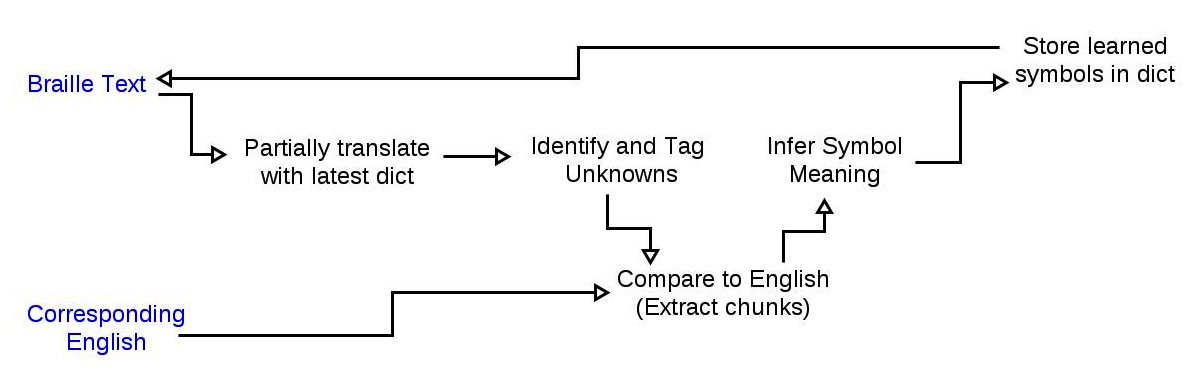
\includegraphics[width = 0.8\columnwidth]{Braillebig}
	\end{figure}
CAMEL learns new symbols by taking 2 input text files (Braille text and corresponding English text), and analyzing them until all unknowns are identified, their meanings are found, and said symbols and their meanings are added to the dictionary.\par}
\vspace{-30pt}
\end{block}

    \begin{block}{{\small Methods of Tagging and Text Extraction}}
%(see \textbf{String Processing Method})
{\tiny
CAMEL must \textit{Tag Unknowns \& Compare to English(Extract Chunks)}  to infer symbol meaning. Four different tag types were used: end, front, mid, and full-word. Below are examples of how these different types of tags were each used to extract meaning. \par}
\begin{figure}\centering
	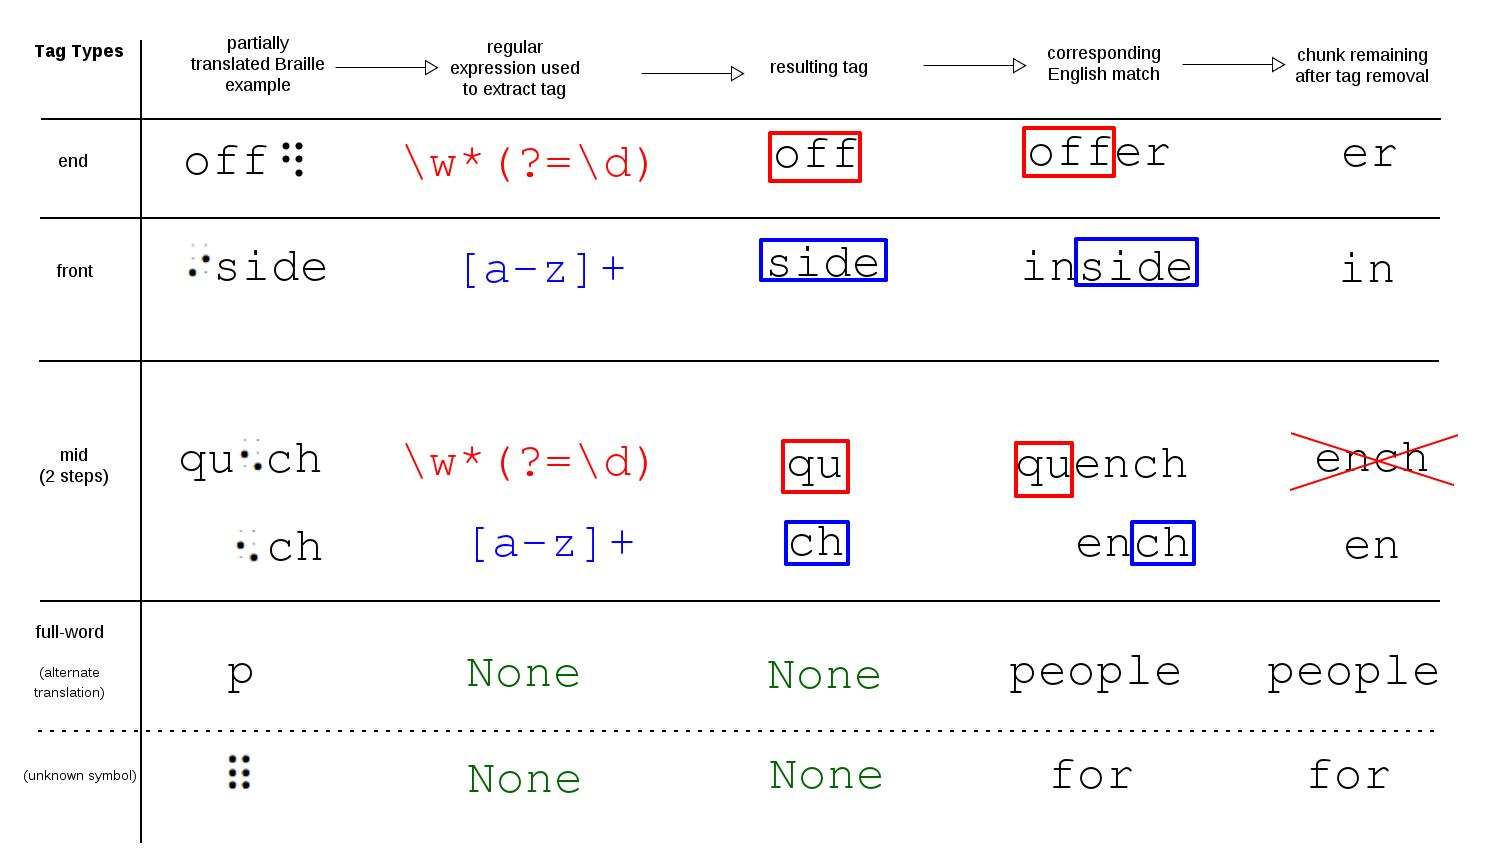
\includegraphics[width=\columnwidth]{taggtypes1}
	\end{figure}
\vspace{-30pt} 
\end{block}
    %\vfill
\begin{block}{{\tiny Acknowledgements}}
\vspace{-10pt}  
{\tiny I'd like to thank: Dr. Marr for introducing me to the beautiful complexity of Computational Semantics; Dr. Jahangeer for her amazing encouragement and her willingness to answer questions; Dr. Borne, Dr. Marr, and Dr. Papaconstantopoulos for supporting me and convincing me to major in Computational and Data Sciences; www.braillebookstore.com for printing and distributing books in Grade 2 Braille, excerpts of which helped train CAMEL.\par}
\end{block}




  \end{column}
  %%%%%%%%%%%%%%%%%%%%%%%%%%%%%%%%%%%%%%%%%%%%%%%%%%%%%%%%%%%%%%%%%%%%%%%%%%%%%%%%%%%%%%%%%%%%%%%%%%%%%%%%%%%%
  %%%%%%%%%%%%%%%%%%%%%%%%%%%%%%%%%%%%%%%%%%%%%%%%%%%%%%%%%%%%%%%%%%%%%%%%%%%%%%%%%%%%%%%%%%%%%%%%%%%%%%%%%%%%
  \begin{column}{.3\linewidth}
   
    %%%%%%%%%%%%%%%%%%%%%%%%%%%%%%%%%%%%%%%%%%%%%%%%%%%%%%%%%%%%%%%%%%%%%%%%%%%%%%%%%%%%%%%%%%%%%%%%%%%%%%%%%%%%

\vspace{-50pt}  
   \begin{block}{{\small Using Contracted Braille As a Platform}}
\vspace{-10pt}  
     {\scriptsize
An example of this process infers the symbols that represent \textit{en} and \textit{in} using the word \textit{penguin} (contracted to \textit{p\{en\}gu\{in\}} in Grade 2 Braille).\par}
          \begin{figure}
	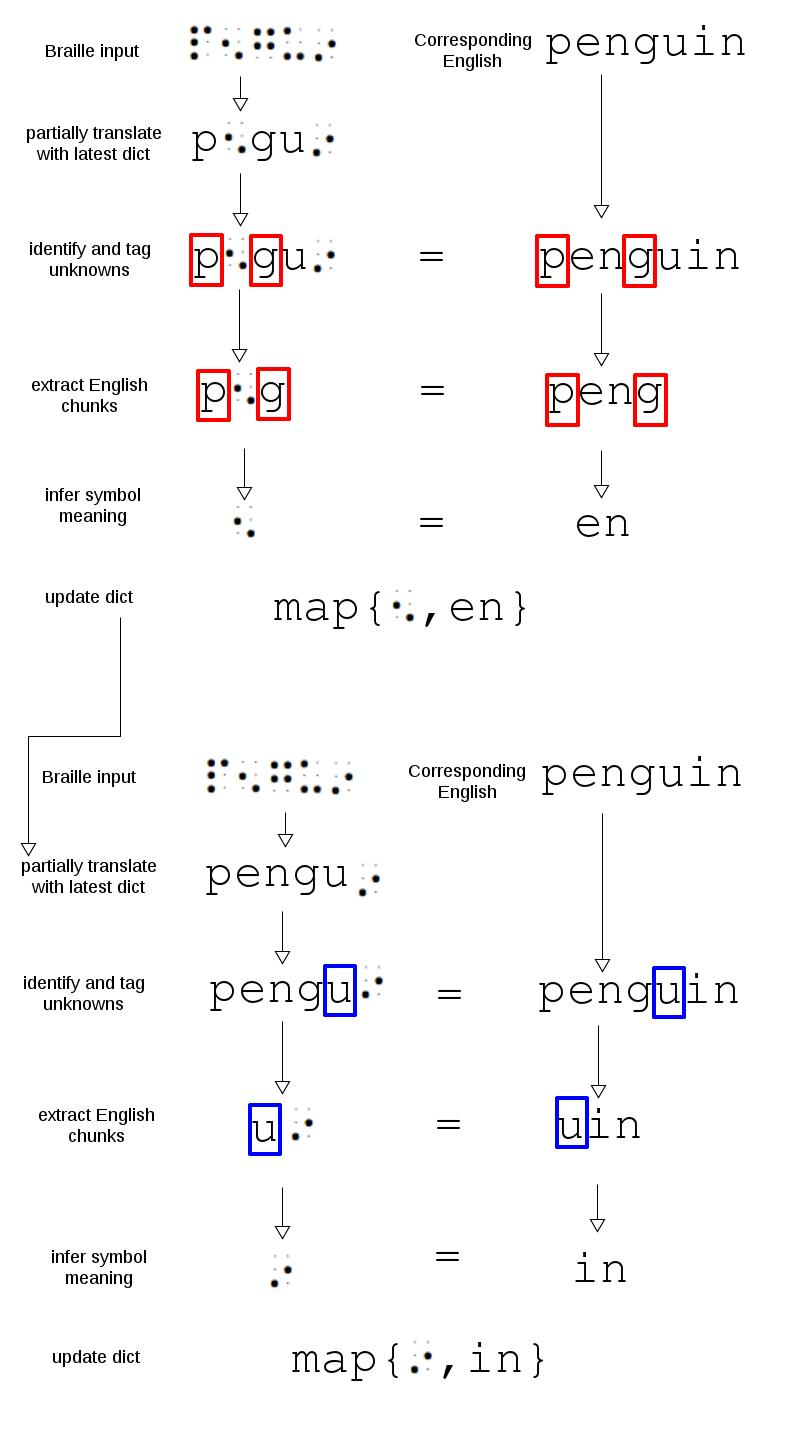
\includegraphics[height = 33cm]{penguin-6}
	\end{figure}
      \end{block}


\begin{block}{{\small Results and Conclusions}}
\vspace{-100pt}
\end{block}
     %%%%%%%%%%%%%%%%%%%%%%%%%%%%%%%%%%%%%%%%%%%%%%%%%%%%%%%%%%%%%%%%%%%%%%%%%%%%%%%%%%%%%%%%%%%%%%%%%%%%%%%%%%%%
      \begin{columns}[t]
        \begin{column}{.505\linewidth}
          %\begin{block}{Safety of Community} 
	{\tiny \textbf{Safety of Community}}
               \begin{itemize}
{\tiny
		\item commercial application in development that will\newline prevent future mislabeling,    such as
	\begin{figure}
	
\includegraphics[width = 0.8\columnwidth]{stairwellmis}
	\end{figure}
 		\item allows sighted people to protect the blind community
\item }
\end{itemize}
         %\end{block}
        \end{column}
        ~
        \begin{column}{.5\linewidth}
          %\begin{block}{Proof of Concept}
	{\tiny \textbf{Proof of Concept}  }
             \begin{itemize}
{\tiny
    		\item $1^{st}$ succesful automated program that learns compressed Braille
		\item translation system is effective for arbitrary symbol systems 
		\item language platform easily changed
\item }
		\end{itemize}
         % \end{block}
        \end{column}
      \end{columns}

  \end{column}
  
  %%%%%%%%%%%%%%%%%%%%%%%%%%%%%%%%%%%%%%%%%%%%%%%%%%%%%%%%%%%%%%%%%%%%%%%%%%%%%%%%%%%%%%%%%%%%%%%%%%%%%%%%%%%%
  %%%%%%%%%%%%%%%%%%%%%%%%%%%%%%%%%%%%%%%%%%%%%%%%%%%%%%%%%%%%%%%%%%%%%%%%%%%%%%%%%%%%%%%%%%%%%%%%%%%%%%%%%%%%
  % !!!!!!!!!!!!!!!    READ ME !
  % Information in the poster footer is declared in the style file. 
  % You must edit beamerthemeSMU.sty

%%%%%%%%%%%%%%%%%%%%%%%%%%%%%%%%%%%%%%%%%%%%%%%%%%%%%%%%%%%%%%%%%%%%%%%%%%%%%%%%%%%%%%%%%%%%%%%%%%%%%%%%%%%%
%%%%%%%%%%%%%%%%%%%%%%%%%%%%%%%%%%%%%%%%%%%%%%%%%%%%%%%%%%%%%%%%%%%%%%%%%%%%%%%%%%%%%%%%%%%%%%%%%%%%%%%%%%%%
%%%%%%%%%%%%%%%%%%%%%%%%%%%%%%%%%%%%%%%%%%%%%%%%%%%%%%%%%%%%%%%%%%%%%%%%%%%%%%%%%%%%%%%%%%%%%%%%%%%%%%%%%%%%
\end{columns}
\end{frame}
\end{document}


